\documentclass{article}

\usepackage{siunitx} % Provides the \SI{}{} and \si{} command for typesetting SI units
\usepackage{graphicx} % Required for the inclusion of images
\usepackage{amsmath} % Required for some math elements 
\usepackage[export]{adjustbox} % loads also graphicx
\usepackage{listings}
\usepackage{matlab-prettifier}
\usepackage{float}

\usepackage{titlesec}
\usepackage{caption}
\usepackage{subcaption}


\usepackage{xcolor}

\DeclareCaptionFont{white}{\color{white}}
\DeclareCaptionFormat{listing}{%
  \parbox{\textwidth}{\colorbox{gray}{\parbox{\textwidth}{#1#2#3}}\vskip-4pt}}
\captionsetup[lstlisting]{format=listing,labelfont=white,textfont=white}
\lstset{frame=lrb,xleftmargin=\fboxsep,xrightmargin=-\fboxsep}
\titleformat{\section}[runin]
  {\normalfont\Large\bfseries}{\thesection}{1em}{}
\titleformat{\subsection}[runin]
  {\normalfont\large\bfseries}{\thesubsection}{1em}{}


\setlength\parindent{0pt} % Removes all indentation from paragraphs

\renewcommand{\labelenumi}{\alph{enumi}.} % Make numbering in the enumerate environment by letter rather than number (e.g. section 6)

%\usepackage{times} % Uncomment to use the Times New Roman font

%----------------------------------------------------------------------------------------
%	DOCUMENT INFORMATION
%----------------------------------------------------------------------------------------

\title{AMATH 353: Homework 1 \\Due April, 4 2018 \\ ID: 1064712} % Title

\author{Trent \textsc{Yarosevich}} % Author name

\date{\today} % Date for the report

\begin{document}
\maketitle % Insert the title, author and date
\setlength\parindent{1cm}

\begin{center}
\begin{tabular}{l r}
%Date Performed: December 1, 2017 \\ % Date the experiment was performed
Instructor: Jeremy Uscal % Instructor/supervisor
\end{tabular}
\end{center}

% If you wish to include an abstract, uncomment the lines below
% \begin{abstract}
% Abstract text
% \end{abstract}

%----------------------------------------------------------------------------------------
%	SECTION 1
%----------------------------------------------------------------------------------------

\section*{Part 1.)}
\subsection*{a.)}
To create a wave moving left with speed one, I used the equation 
\begin{equation}
u(x,t) = exp(-x - ct)^2) 
\end{equation}
with $c = -1$. The following figure displays its movement to the left over time with a speed of 1.
\begin{figure}[H]
\centering
    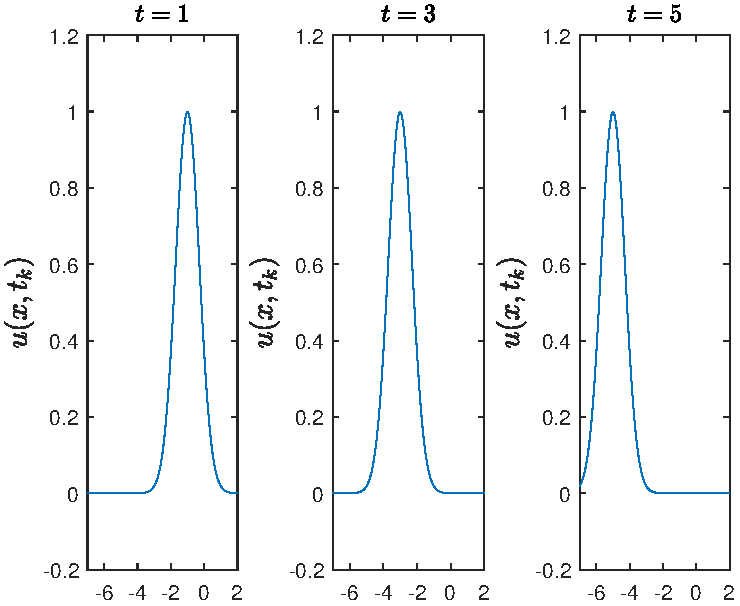
\includegraphics[width=75mm, scale=.8]{plot_1a.pdf}
	\caption{Moving left with speed 1.}
\end{figure}
\subsection*{b.) and c.)}
Parts b.) and c.) were executed with the following values for $c$ in the same equation used on part a.), which I have accompanied with visualizations. Note that the 'speed' is displayed by the identical figures and increasing or decreasing x-axes.
\begin{figure}[H]
\centering
    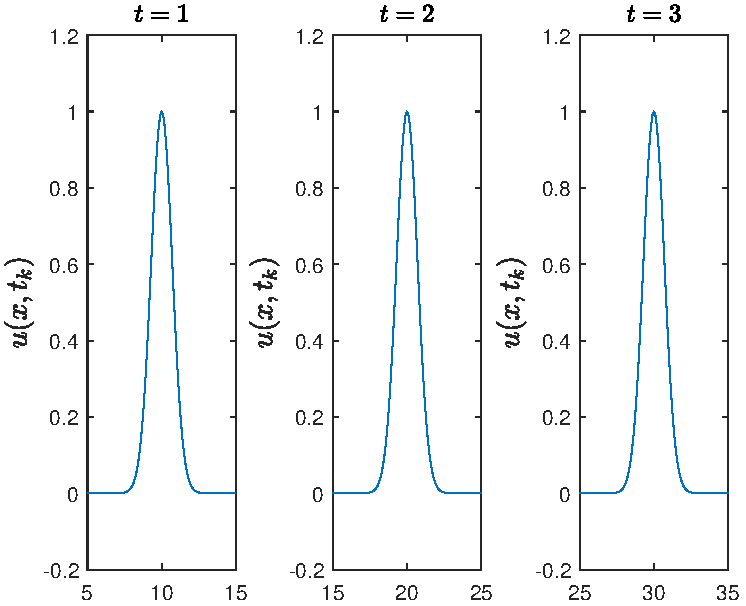
\includegraphics[width=75mm, scale=.8]{plot_1b.pdf}
	\caption{$c = 10$, moving right with speed 10.}
\end{figure}
\begin{figure}[H]
\centering
    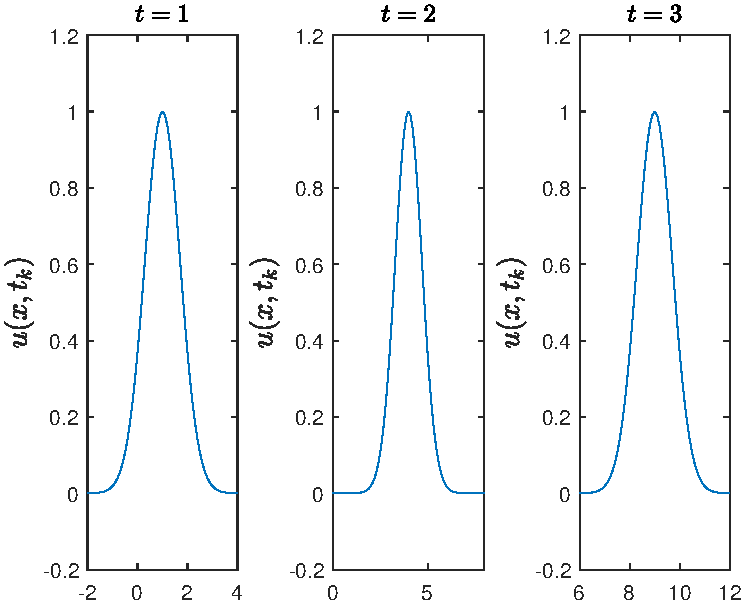
\includegraphics[width=75mm, scale=.8]{plot_1c.pdf}
	\caption{$c = t$, moving right with speed $t$.}
\end{figure}
\subparagraph*{d.)} Part d.) modifies the equation in a.) to implement decreasing amplitude inversely proportional to $t$.
\begin{equation}
u(x,t) = \frac{1}{t}exp(-x - ct)^2) 
\end{equation}

\begin{figure}[H]
\centering
    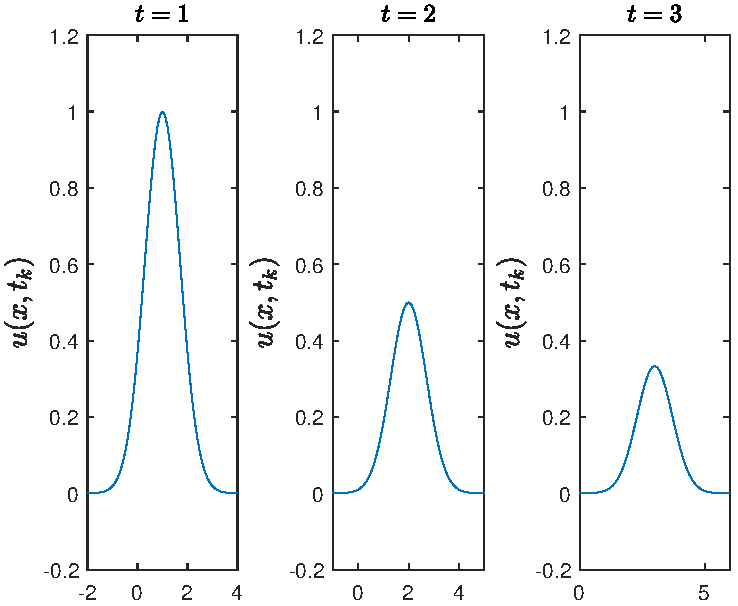
\includegraphics[width=75mm, scale=.8]{plot_1d.pdf}
	\caption{$c = 10$, moving right with speed 1 and amplitude inversely proportional to $t$.}
\end{figure}
\section*{Part 2.)}
\subsection*{a.)} 
$v_{tt} - v_{xxx} = 0$
\subsection*{b.)}
Let $\alpha = \beta = 1$\\

\noindent By linear differential operators, 
\begin{equation}
\begin{aligned}
u_{3, tt} = u_{3, xxx} \\
(u_{1} + u_{2})_{tt} = (u_{1} + u_{2})_{xxx}\\
u_{1, tt} + u_{2, tt} = u_{1, xxx} + u_{2, xxx}\\
u_{1, tt} + u_{2, tt} - u_{1, xxx} - u_{2, xxx} = 0\\
u_{1, tt} - u_{1, xxx} + u_{2, tt} - u_{2, xxx} = 0\\
\end{aligned}
\end{equation}
Thus as hoped after plugging in $u_{3}$ we arrive at the sum of two homogeneous equations of the solutions $u_1$ and $u_2$.
\subsection*{c.)}
$v_{tt} + vv_{xxx} = 0$\\

\subsection*{d.)}
\begin{equation}
\begin{aligned}
u_{3, tt} + u_3u_{3,xxx} = 0\\
(u_1 + u_2)_{tt} + (u_1 + u_2)(u_1 + u_2)_{xxx} = 0\\
u_{1, tt} + u_{2, tt} + u_1u_{1, xxx} + u_1u_{2, xxx} + u_2u_{1, xxx} + u_2u_{2, xxx} = 0\\
\end{aligned}
\end{equation}
And then, because $v_{tt} + vv_{xxx} = 0$ for both solutions $u_1$ and $u_2$, we are left with
\begin{equation}
\begin{aligned}
u_1u_{2, xxx} + u_2u_{1, xxx} = 0\\
\end{aligned}
\end{equation}
which only holds true for certain special cases of $u_1$ and $u_2$.
\subsection*{e.)}
$v_{tt} + kv_t + v_{xxx} = 0$ with some dampening constant $k$.
\subsection*{f.)}
Boundary conditions: $v(a, t) = v(b, t) = 0, v_x(a,t) = 1$ for $t > 0$.\\
Initial values: $v(x, t_0) = f(x)$ and $v_t(x, t_0) = g(x)$.
\section*{Part 3.)}
\subsection*{a.)}
Both $f_2$ and $f_3$ satisfy periodic boundary conditions. 
\subsection*{b.)}
Only $f_1$ satisfies decaying boundary conditions as the limit of $\lvert x\rvert$ approaches $\infty$.
\section*{Part 4.)}
The prompt is essentially asking which equations are both homogeneous and linear. The equations a.), c.) and d.) are linear and homogeneous, and therefore two solutions can be added together, with constants $c_1$ and $c_2$ equal to 1, to provide a third solution, in this case $u$. This does not hold for b.) because the $e^{-t}$ term means it is not homogeneous, resulting in a clearly untrue statement when we plug in $u_3$ and expand: $2e^{-t} = e^{-t}$. This also does not hold for e.) or f.) because of the non-linear terms $sin(u)$ and $uu_x$ respectively, which lead to results similar to those demonstrated above in 2.d.).
\end{document}
